\chapter{Dérivation - Partie 2}
\thispagestyle{fancy}

\section{Fonction dérivée}
\begin{definition}
	La fonction qui à tout réel $x$ associe le nombre dérivé de $f$ en $x$ est appelée fonction dérivée de $f$ et se note $f^{\prime}$.
\end{definition}
	


\subsection*{Formules de dérivation de fonctions usuelles}

\begin{center}
	\begin{tabular}{|c|c|}
		\hline
		Fonction & Dérivée \\
		\hline
		$f(x)=a, a \in \mathbb{R}$ & $f^{\prime}(x)=0$ \\
		\hline
		$f(x)=a x, a \in \mathbb{R}$ & $f^{\prime}(x)=a$ \\
		\hline
		$f(x)=x^{2}$ & $f^{\prime}(x)=2 x$ \\
		\hline
		$f(x)=x^{3}$ & $f^{\prime}(x)=3 x^{2}$ \\
		\hline
	\end{tabular}
\end{center}

\subsection*{Formules d'opération sur les fonctions dérivées}

$$
\begin{gathered}
	(f+g)^{\prime}=f^{\prime}+g^{\prime} \\
	(k f)^{\prime}=k f^{\prime} \quad k \in \mathbb{R}
\end{gathered}
$$

\begin{methodeTitre}{Calculer des fonctions dérivées}
	\grasInMet{Enoncé :}
	
Dans chaque cas, calculer la fonction dérivée de la fonction $f$ :
\begin{enumMet}
\begin{multicols}{2}
	\item $f(x)=3 x$
	\item $f(x)=x^{2}+5$
	\item $f(x)=5 x^{3}$
	\item $f(x)=3 x^{2}+4 x$	
\end{multicols}
	
\end{enumMet}

\grasInMet{Solution :}
\begin{enumMet}
	\begin{multicols}{2}
		\item $f^{\prime}(x)=3$
		\item $f^{\prime}(x)=2 x+0=2 x$
		\item $f^{\prime}(x)=5 \times 3 x^{2}=15 x^{2}$
		\item $f^{\prime}(x)=3 \times 2 x+4=6 x+4$
	\end{multicols}
	
\end{enumMet}
\end{methodeTitre}

\section{Fonction dérivée d'une fonction polynôme}

\subsection{Fonction polynôme de degré 2}

Soit $f$ une fonction polynôme du second degré définie par $f(x)=5 x^{2}-3 x+2$.\\
Pour déterminer la fonction dérivée $f^{\prime}$, on applique la technique suivante :

$$
\begin{aligned}
	f(x)&=5 \times x^{2}-3 x+2 \\
	& \downarrow \\
	f^{\prime}(x)&=5 \times 2 x-3+0 \\
	&=10 x-3
\end{aligned}
$$

\begin{definition}
	Soit f une fonction polynôme du second degré définie sur \R par
	$f(x)=ax^2+bx+c$.\\
	\ \\
	On appelle fonction dérivée de $f$, notée $f^{\prime}$, la fonction définie sur \R par $f^{\prime}(x)=a \times 2 x+b$.
\end{definition}

\begin{methodeTitre}{Déterminer la fonction dérivée d'une fonction polynôme du second degré}
	\grasInMet{Enoncé :}
	
	Déterminer les fonctions dérivées des fonctions suivantes:
	\begin{enumMet}
		\begin{multicols}{2}
			\item $f(x)=4 x^{2}-6 x+1$
			\item $g(x)=-3 x^{2}+2 x+8$
			\item $h(x)=-x^{2}+7 x$
		\end{multicols}
		
	\end{enumMet}
	
	\grasInMet{Solution :}
	\begin{enumMet}
		\begin{multicols}{2}
			\item $f^{\prime}(x)=4 \times 2 x-6+0=8 x-6$
			\item $g^{\prime}(x)=(-3) \times 2 x+2=-6 x+2$
			\item $h^{\prime}(x)=-2 x+7$
		\end{multicols}
	\end{enumMet}
\end{methodeTitre}

\subsection{Fonction polynôme de degré 3}
Soit $f$ une fonction polynôme du troisième degré définie par:\\
$f(x)=2 x^{3}-3 x^{2}+5 x-1$.\\
Pour déterminer la fonction dérivée $f^{\prime}$, on applique la technique suivante :

$$
\begin{aligned}
	f(x)&=2 \times x^{3}-3 \times x^{2}+5 x-1 \\
	& \downarrow \\
	f^{\prime}(x)&=2 \times 3 x^{2}-3 \times 2 x+5-0 \\
	&=6 x^{2}-6 x+5
\end{aligned}
$$

\begin{definition}
	Soit $f$ une fonction polynôme du troisième degré définie sur $\mathbb{R}$ par
	$f(x)=a x^{3}+b x^{2}+c x+d$.
	
	\ \\
	
	On appelle fonction dérivée de $f$, notée $f^{\prime}$, la fonction définie sur $\mathbb{R}$ par $$f^{\prime}(x)=a \times 3 x^{2}+b \times 2 x+c$$
\end{definition}


\begin{methodeTitre}{Déterminer la fonction dérivée d'une fonction polynôme du troisième degré}
	\grasInMet{Enoncé :}
	
	Déterminer les fonctions dérivées des fonctions suivantes:
	\begin{enumMet}
		\begin{multicols}{2}
			\item $f(x)=5 x^{3}+2 x^{2}+2 x-7$
			\item $g(x)=-2 x^{3}-3 x^{2}-7 x+8$
			\item $h(x)=4 x^{3}+1$
		\end{multicols}
		
	\end{enumMet}
	
	\grasInMet{Solution :}
	\begin{enumMet}
			\item $f^{\prime}(x)=5 \times 3 x^{2}+2 \times 2 x+2=15 x^{2}+4 x+2$
			\item $g^{\prime}(x)=(-2) \times 3 x^{2}-3 \times 2 x-7=-6 x^{2}-6 x-7$
			\item $h^{\prime}(x)=4 \times 3 x^{2}=12 x^{2}$	
	\end{enumMet}
\end{methodeTitre}

\section{Variations d'une fonction polynôme}

\begin{theoreme}
	\begin{itemDef}
		\item Si $f^{\prime}(x) \leq 0$, alors $f$ est décroissante.
		\item Si $f^{\prime}(x) \geq 0$, alors $f$ est croissante.
	\end{itemDef}
\end{theoreme}
\section*{Théorème:}

\begin{methodeTitre}{Étudier les variations d'une fonction polynôme du second degré}
	\grasInMet{Enoncé :}
	
	Soit la fonction $f$ définie sur $\mathbb{R}$ par $f(x)=2 x^{2}-8 x+1$.
	\begin{enumMet}
		\item Calculer la fonction dérivée de $f$.
		\item Déterminer le signe de $f'$ en fonction de $x$.
		\item Dresser le tableau de variations de $f$.
	\end{enumMet}
	
	\grasInMet{Solution :}
	\begin{enumMet}
		\item $f^{\prime}(x)=2 \times 2 x-8=4 x-8$.
		\item Étude du signe de la dérivée :
		
		On commence par résoudre l'équation $f^{\prime}(x)=0$.\\
		Soit : $4 x-8=0$
		
		$$
		\begin{aligned}
			& 4 x=8 \\
			& x=\frac{8}{4}=2 .
		\end{aligned}
		$$
		
		La fonction $f^{\prime}$ est une fonction affine représentée par une droite dont le coefficient directeur 4 est positif.\\
		Donc $f^{\prime}$ est croissante. Elle est donc d'abord négative (avant $x=2$ )\\
		puis positive (après $x=2$ ).
		\item On dresse le tableau de variations en appliquant le théorème :
		\begin{center}
			\begin{tikzpicture}
				\tkzTabInit{$x$ / 1 , $f'(x)$ / 1, $f(x)$ / 1.5}{$-\infty$, $2$, $+\infty$}
				\tkzTabLine{, -, z, +, }
				\tkzTabVar{+/ , -/ $-7$, +/ }
			\end{tikzpicture}
		\end{center}
		$$
		f(2)=2 \times 2^{2}-8 \times 2+1=-7 .
		$$
		
		La fonction $f$ admet un minimum égal à -7 en $x=2$.
	\end{enumMet}
\end{methodeTitre}

\begin{methodeTitre}{Étudier les variations d'une fonction polynôme du troisième degré}
	\grasInMet{Enoncé :}
	
	Soit la fonction $f$ définie sur \R par $f(x)=x^{3}+\dfrac{9}{2} x^{2}-12 x+5$.
	\begin{enumMet}
		\item \begin{enumMet}
			\item Calculer la fonction dérivée de $f$.
			\item Démontrer que $f^{\prime}(x)=3(x+4)(x-1)$.
		\end{enumMet}
		\item Déterminer le signe de $f^{\prime}$ en fonction de $x$.
		\item Dresser le tableau de variations de $f$.
	\end{enumMet}
	
	\grasInMet{Solution :}
	\begin{enumMet}
		\item \begin{enumMet}
			\item On a:\\
			$f^{\prime}(x)=3 x^{2}+\dfrac{9}{2} \times 2 x-12=3 x^{2}+9 x-12$
			\item Développons $3(x+4)(x-1)$ :\\
			$3(x+4)(x-1)$\\
			$=(3 x+12)(x-1)$\\
			$=3 x^{2}-3 x+12 x-12$\\
			$=3 x^{2}+9 x-12$\\
			$=f^{\prime}(x)$\\
			Donc $f^{\prime}(x)=3(x+4)(x-1)$.
		\end{enumMet}
		\begin{minipage}[c]{0.74\linewidth}
			\item On commence par résoudre l'équation $f^{\prime}(x)=0$ :\\
			$3(x+4)(x-1)=0$\\
			$x+4=0 \quad$ ou $\quad x-1=0$\\
			$x=-4 \quad x=1$
			
			La dérivée s'annule en $-4$ et 1 .\\
			Comme $a=3>0$, les branches de la parabole représentant la fonction dérivée sont tournées vers le haut (position \Smiley{}).\\
			La dérivée est donc d'abord positive, puis négative, puis positive.\\
		\end{minipage} \hfill
		\begin{minipage}[c]{0.25\linewidth}
			
\includegraphics[scale=0.35]{2025_01_20_261e7c883d9fae066150g-5(1)}
		\end{minipage}
		
		\item On en déduit le tableau de variations de $f$ :\\
		\begin{center}
			\begin{tikzpicture}
				\tkzTabInit{$x$ / 1 , $f'(x)$ / 1, $f(x)$ / 1.5}{$-\infty$, $-4$,$1$, $+\infty$}
				\tkzTabLine{, +, z,-,z, +, }
				\tkzTabVar{-/ ,+/61, -/ $-\dfrac{3}{2}$, +/ }
			\end{tikzpicture}
		\end{center}
		En effet :\\
		$f(-4)=(-4)^{3}+\dfrac{9}{2} \times(-4)^{2}-12 \times(-4)+5=61$\\
		$f(1)=1^{3}+\dfrac{9}{2} \times 1^{2}-12 \times 1+5=-\dfrac{3}{2}$\\
	\end{enumMet}
\end{methodeTitre}







